\documentclass[lualatex,ja=standard,a4paper,11pt]{bxjsarticle}

\usepackage{luatexja}
\usepackage{amsmath,amssymb}
\usepackage{graphicx}
\usepackage{xcolor}
\usepackage{url}
\usepackage{booktabs}
\geometry{reset,margin=25mm}
\usepackage[unicode,hidelinks]{hyperref}

\renewcommand{\figurename}{図}
\renewcommand{\tablename}{表}
\renewcommand{\refname}{参考文献}

\title{文学的感情理解のための日本語人間評価に基づくベンチマークと多言語ロバスト性検証}
\author{%
Naruki Shirahama\\
下関市立大学\\
下関市, 山口県, 日本\\
\url{nshirahama@ieee.org}
\and
Yuma Yoshimoto\\
北九州工業高等専門学校\\
北九州市, 福岡県, 日本\\
\url{yoshimoto@kct.ac.jp}
\and
Naofumi Nakaya\\
順天堂大学\\
浦安市, 千葉県, 日本\\
\url{n.nakaya.ac@juntendo.ac.jp}
\and
Junji Nishino\\
玉川大学\\
町田市, 東京都, 日本\\
\url{nishinojunji@eng.tamagawa.ac.jp}
\and
Satoshi Watanabe\\
静岡理工科大学\\
袋井市, 静岡県, 日本\\
\url{satoshi\_watanabe@ieee.org}
}
\date{}

\begin{document}

\maketitle

\begin{center}
\small
\textit{Proc. of the International Conference on Electrical, Computer, Communications and Mechatronics Engineering (ICECCME 2026), 15--17 October 2026, Bali, Indonesia}
\end{center}

\begin{abstract}
感情的テキスト理解に関する大規模言語モデル（LLM）評価では、人間評価に基づく検証が依然として中心的な課題である。既存のベンチマークや多言語プロファイリングは、モデル間または言語間の差異を明らかにできる一方で、その差異だけでは、どのシステムが人間の判断に近いかを示すことはできない。本論文では、日本文学作品3編と、興味、驚き、悲しみ、怒りの4つの連続的感情次元を用いた、コンパクトな人間評価基盤の多言語ベンチマークを提案する。学生読者による日本語Visual Analogue Scale（VAS）評定を参照プロファイルとし、統一されたマルチプロバイダ実験基盤を通じて、現代的な6種類のLLMを比較する。主要評価項目は、中立的読者プロンプトのもとでの日本語人間参照との整合性であり、英語および中国語条件は、同等の人間評価エンドポイントではなく、言語横断ドリフトに関するロバスト性検証として扱う。Claude Sonnet 4.5は、日本語人間参照に対する平均絶対誤差が最小（20.026）であった一方、Gemini 2.5 Proは最大の誤差（28.952）を示した。GPT-5.4は人間プロファイルとの順位一致が最も高く、Qwen3.6 PlusとGPT-5.4は平均言語横断ドリフトが最小（それぞれ3.346および3.354）であった。これらの結果は、主要な人間整合性と多言語ロバスト性が関連しつつも分離可能な性質であることを示しており、本ベンチマークがコンパクトで再現可能なモデル選別に有用であることを示唆する。
\end{abstract}

\noindent\textbf{キーワード:}
大規模言語モデル, 人間評価基盤評価, 文学的感情理解, 多言語ロバスト性, Visual Analogue Scale

\section{はじめに}

感情的テキスト理解に関するLLM評価では、ベンチマークスイート、多言語テスト、人間とAIの比較が広く用いられるようになっている。これらの手法は有用であるが、重要な評価項目の階層が十分に明示されていない場合が多い。すなわち、モデル間または言語間の差異は出力が異なることを示せるものの、その出力が人間の判断に近いかどうかは示せない。一方で、小規模な人間対AI比較は、単一モデルまたは単一言語条件に焦点を当てることが多い\cite{shirahama2025vas,paech2024eqbench,huang2024emotionbench}。したがって、コンパクトなベンチマークが有用であるためには、人間参照を明示的に維持し、多言語安定性を人間妥当性の代替として扱わないことが必要である。

本論文は、日本語VAS人間評定を参照プロファイルとして用い、日本語条件を主要評価項目として扱うことで、この課題に取り組む。英語および中国語は、言語横断ドリフトに関するロバスト性条件としてのみ分析する。したがって、本研究の貢献は一般的な言語効果の研究ではなく、日本語人間参照との主要な整合性と、副次言語におけるロバスト性を分離する、コンパクトな人間評価基盤フレームワークにある。

本論文の具体的な貢献は3点である。第一に、主要な主張を日本語人間参照データに明確に固定した、再現可能なベンチマーク設計を提示する。第二に、人間整合性と多言語ロバスト性を分離し、副次言語での挙動を人間妥当性の代替として過度に解釈しない評価枠組みを示す。第三に、大規模な多言語研究またはマルチペルソナ研究に進む前のコンパクトな工学的評価として実用的な、日本語較正と言語横断ドリフトの二軸スクリーニング視点を提供する。

\section{関連研究}

本研究は、4つの研究系譜の交点に位置する。第一は、人間とAIの感情判断を比較し、粗いカテゴリラベルではなく連続尺度を用いる意義を示す研究である。我々の先行研究であるVASとLikert尺度の比較では、短編小説の感情評価においてVASベースの設計が実用的であり、小さな離散尺度よりも精密な人間--LLM比較の基盤として適していることを示した\cite{shirahama2025vas}。

第二は、LLMの感情知能に関するベンチマーク設計である。EQ-Bench、EmotionBench、EmoBench、EmotionQueenなどのベンチマークスイートは、感情推論、共感、感情的応答品質の評価を標準化する上で重要な役割を果たしてきた\cite{paech2024eqbench,huang2024emotionbench,sabour2024emobench,chen2024emotionqueen}。しかし、これらのスイートは、連続的な物語別・感情別スコアリングを用いた文学読解課題において、現行モデルのどれが人間参照プロファイルに最も近いかを問うことを主目的として設計されたものではない。

第三は、多言語およびロバスト性志向のLLM評価である。言語の変更は、語彙選択、物語のフレーミング、較正に影響を与え得るため、翻訳条件を含む展開を想定するベンチマークでは多言語比較が必要となる。しかし、対応する人間参照が利用できない限り、多言語変動それ自体は人間妥当性と同義ではない。

第四は、我々自身のプラットフォーム開発および数理的特徴づけに関する先行研究である。これらの研究では、広範なモデル群において、LLMの信頼性、制御可能性、感情的個性が大きく異なることを示した\cite{openrouterplatform,shirahama2026mdpi}。本論文では意図的に設計を絞り、一つの中立的読者条件、一つの人間評価に基づく言語エンドポイント、そして直接的な人間検証の代替ではなくロバスト性分析として解釈される多言語実行に焦点を当てる。

\section{データと方法}

\textbf{人間参照データ.}
本ベンチマークでは、3編の日本語短編文学テキストと、興味、驚き、悲しみ、怒りの4つの感情次元に対する回答者レベルのVASデータを用いる。対象作品は、夢野久作「懐中時計」（T1）、夢野久作「お金とピストル」（T2）、高村光太郎「ぼろぼろな駝鳥」（T3）である。課題は学生読者に対して日本語VAS調査として実施され、各回答者は各作品を読んだ後、同じ4感情について評定した。人間回答は91件収集され、そのうち86件の完全回答を主要な集約参照プロファイルとして保持した。公開リポジトリには匿名化・サニタイズ済みの数値派生データのみを保存している。本分析では、学生VASデータから得られた匿名化済み二次数値派生物のみを再利用し、元の調査エクスポートやプラットフォームメタデータは再配布しない。

\textbf{テキストとモデル群.}
計算ベンチマークでは、人間課題で使用した同じ3作品を評価対象とし、6つの主要プロバイダから選んだ現代的な6種類のLLM、すなわちClaude Sonnet 4.5、GPT-5.4、Grok 4.20、Qwen3.6 Plus、DeepSeek V3.2、Gemini 2.5 Proを比較する。各モデルは日本語、英語、中国語で問い合わせられた。モデル群は、ベンダ多様性を維持しつつ、本論文の工学的パイロット研究としての範囲に合わせてコンパクトに設定した。

\textbf{課題定義.}
中立的読者モデル実行では、人間VAS課題に近づけるため、同じ4つの感情次元を0--100尺度で操作化した。1つのLLM実験単位は、1モデル、1言語、1作品、1つの中立的読者プロンプト、1反復からなる。モデルには、文学テキスト全文、中立的読者としての役割、4感情の定義、0はその感情をまったく感じない、50は中程度に感じる、100は非常に強く感じるという採点規則を与えた。出力は、4つの整数スコアと、テキストに基づく簡潔な理由を含む1つのJSONオブジェクトとした。ベンチマークをペルソナ条件付き評価ではなく、人間整合性のパイロットとして解釈可能に保つため、すべての言語で単一の中立的読者プロンプトを用いた。参照VASデータは日本語で収集されており、日本語原文と日本語の課題指示が主要な人間--LLM整合性条件で使用されたため、日本語人間整合性を主要評価項目とした。したがって、英語と中国語は同等の人間評価に基づく評価としてではなく、言語横断ロバスト性検証として扱う。これらの実行では、文学テキストと課題指示の双方を、著者が固定した翻訳により言語を一致させたため、観測されるドリフトは指示言語だけでなく、翻訳されたテキストとプロンプト言語の複合的影響を反映する。本ベンチマークは意図的にコンパクトであるため、分析は形式的な有意性検定ではなく、スクリーニングの有用性を目的とした記述的比較として解釈する。この設計では、先行するLLMのみの設計においてペルソナと温度が交絡していたことを踏まえ\cite{shirahama2026mdpi}、ペルソナ条件付きプロンプティングを本論文の中心から外している。

\begin{figure}[t]
\centering
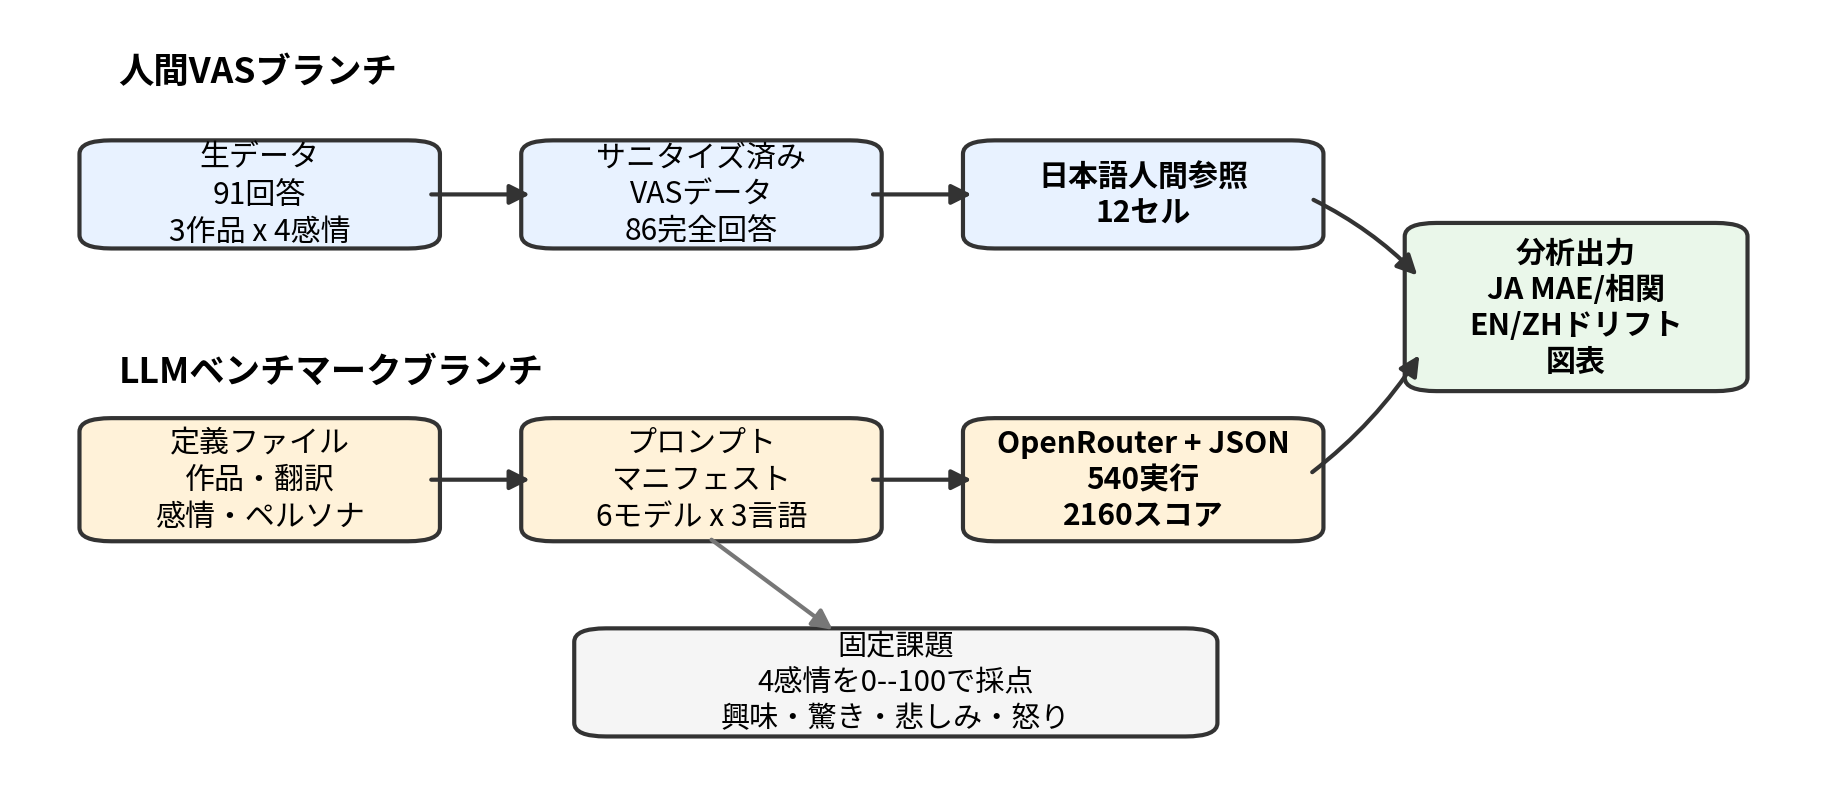
\includegraphics[width=0.98\textwidth]{fig/figure1_system_workflow_ja.pdf}
\caption{本ベンチマークのシステム構成とデータフロー。人間ブランチでは、非公開の日本語VASワークブックをサニタイズ済みの物語別・感情別参照セルへ変換する。LLMブランチでは、固定された定義ファイル、翻訳テキスト、プロンプトテンプレート、応答スキーマ、モデルマニフェストを組み合わせ、OpenRouterを通じて中立的読者ベンチマークを実行する。分析では、日本語モデルプロファイルを人間参照と比較し、英語および中国語を言語横断ロバスト性条件として扱う。}
\label{fig:workflow}
\end{figure}

\textbf{集約.}
$s \in \{1,2,3\}$をテキストのインデックス、$d \in \{1,2,3,4\}$を感情次元のインデックスとする。日本語人間参照プロファイルは次式で定義される。
\begin{equation}
H_{s,d}=\frac{1}{N_s}\sum_{i=1}^{N_s} y_{i,s,d},
\end{equation}
ここで、$y_{i,s,d}$は回答者$i$によるVASスコア、$N_s$はテキスト$s$に対する完全回答数である。モデル$m$、言語$\ell \in \{\mathrm{JA},\mathrm{EN},\mathrm{ZH}\}$、反復回数$R=10$について、集約モデルプロファイルは次式で表される。
\begin{equation}
M_{m,\ell,s,d}=\frac{1}{R}\sum_{r=1}^{R} x_{m,\ell,s,d,r}.
\end{equation}
これにより、各モデル・言語条件について、12値からなる物語別・感情別プロファイルが得られる。

\textbf{評価指標.}
主要評価項目は日本語人間整合性である。各モデルについて、日本語スコアを物語別・感情別プロファイルに集約し、日本語人間参照と平均絶対誤差（MAE）、Pearson相関、Spearman順位相関により比較した。
\begin{equation}
\mathrm{MAE}_{m,\mathrm{JA}}=\frac{1}{12}\sum_{s,d}\left|M_{m,\mathrm{JA},s,d}-H_{s,d}\right|.
\end{equation}
英語と中国語は追加の人間評価エンドポイントとしては扱わない。代わりに、言語横断ドリフトを、各モデルの英語または中国語の物語別・感情別スコアプロファイルと、同じモデルの日本語プロファイルとの平均絶対差として定義した。
\begin{equation}
D_{m,\ell}=\frac{1}{12}\sum_{s,d}\left|M_{m,\ell,s,d}-M_{m,\mathrm{JA},s,d}\right|,~~
\ell \in \{\mathrm{EN},\mathrm{ZH}\}.
\end{equation}
さらに、平均ドリフトを次式で報告する。
\begin{equation}
\bar{D}_m=\frac{D_{m,\mathrm{EN}}+D_{m,\mathrm{ZH}}}{2}.
\end{equation}
MAEとドリフトはいずれも低いほど望ましい。本ベンチマークは意図的にコンパクトであるため、論文では形式的な有意性検定ではなく、記述的比較とスクリーニング有用性を重視する。

\textbf{プロトコルと再現性.}
プロトコルは、91件の人間回答、主要な集約参照プロファイルに保持された86件の完全回答、3テキスト、4感情次元から構成される。モデル側では、1つの中立的読者プロンプトのもとで、6モデル $\times$ 3言語 $\times$ 3テキスト $\times$ 10反復を扱い、合計540件の中立的読者モデル実行と2160個の数値スコアを得た。図~\ref{fig:workflow}に、2つのデータブランチと下流分析の流れを示す。再現性のため、公開リポジトリには学生VASデータのサニタイズ済み数値派生物のみを保存し、元の調査エクスポートやプラットフォームメタデータは再配布しない。

\begin{table}[t]
\caption{主要ベンチマーク設計の概要}
\label{tab:design}
\centering
\begin{tabular}{lr}
\toprule
項目 & 値 \\
\midrule
人間回答数 & 91 \\
完全回答数 & 86 \\
テキスト数 & 3 \\
感情次元数 & 4 \\
モデル数 & 6 \\
言語数 & 3 (JA/EN/ZH) \\
プロンプト条件 & 1 (中立的読者) \\
各条件の反復回数 & 10 \\
中立的読者モデル実行総数 & 540 \\
数値スコア総数 & 2160 \\
\bottomrule
\end{tabular}
\end{table}

\section{結果}

図~\ref{fig:workflow}にシステム構成とデータフローを示し、表~\ref{tab:design}にベンチマーク設計の概要を示す。図~\ref{fig:ja-ranking}は日本語人間整合性ランキングを、図~\ref{fig:drift}は日本語に対する言語横断ドリフトを示す。表~\ref{tab:primary}は主要な要約統計量を報告し、図~\ref{fig:tradeoff}は二軸スクリーニング視点を可視化する。

\textbf{日本語人間整合性.}
主要な日本語条件において、Claude Sonnet 4.5は人間参照に対する平均絶対誤差（MAE）が最小（20.026）であり、DeepSeek V3.2（20.100）、Qwen3.6 Plus（20.744）、GPT-5.4（21.113）、Grok 4.20（21.410）がこれに続いた。一方、Gemini 2.5 Proは最大の誤差（28.952）を示した。最良モデルと最下位モデルの差は8.926点であった。同時に、上位4モデルはわずか1.087 MAE点以内に密集しており、強いモデル群の内部では、比較的小さな較正差がモデル選別に影響し得ることを示している。

\begin{figure}[t]
\centering
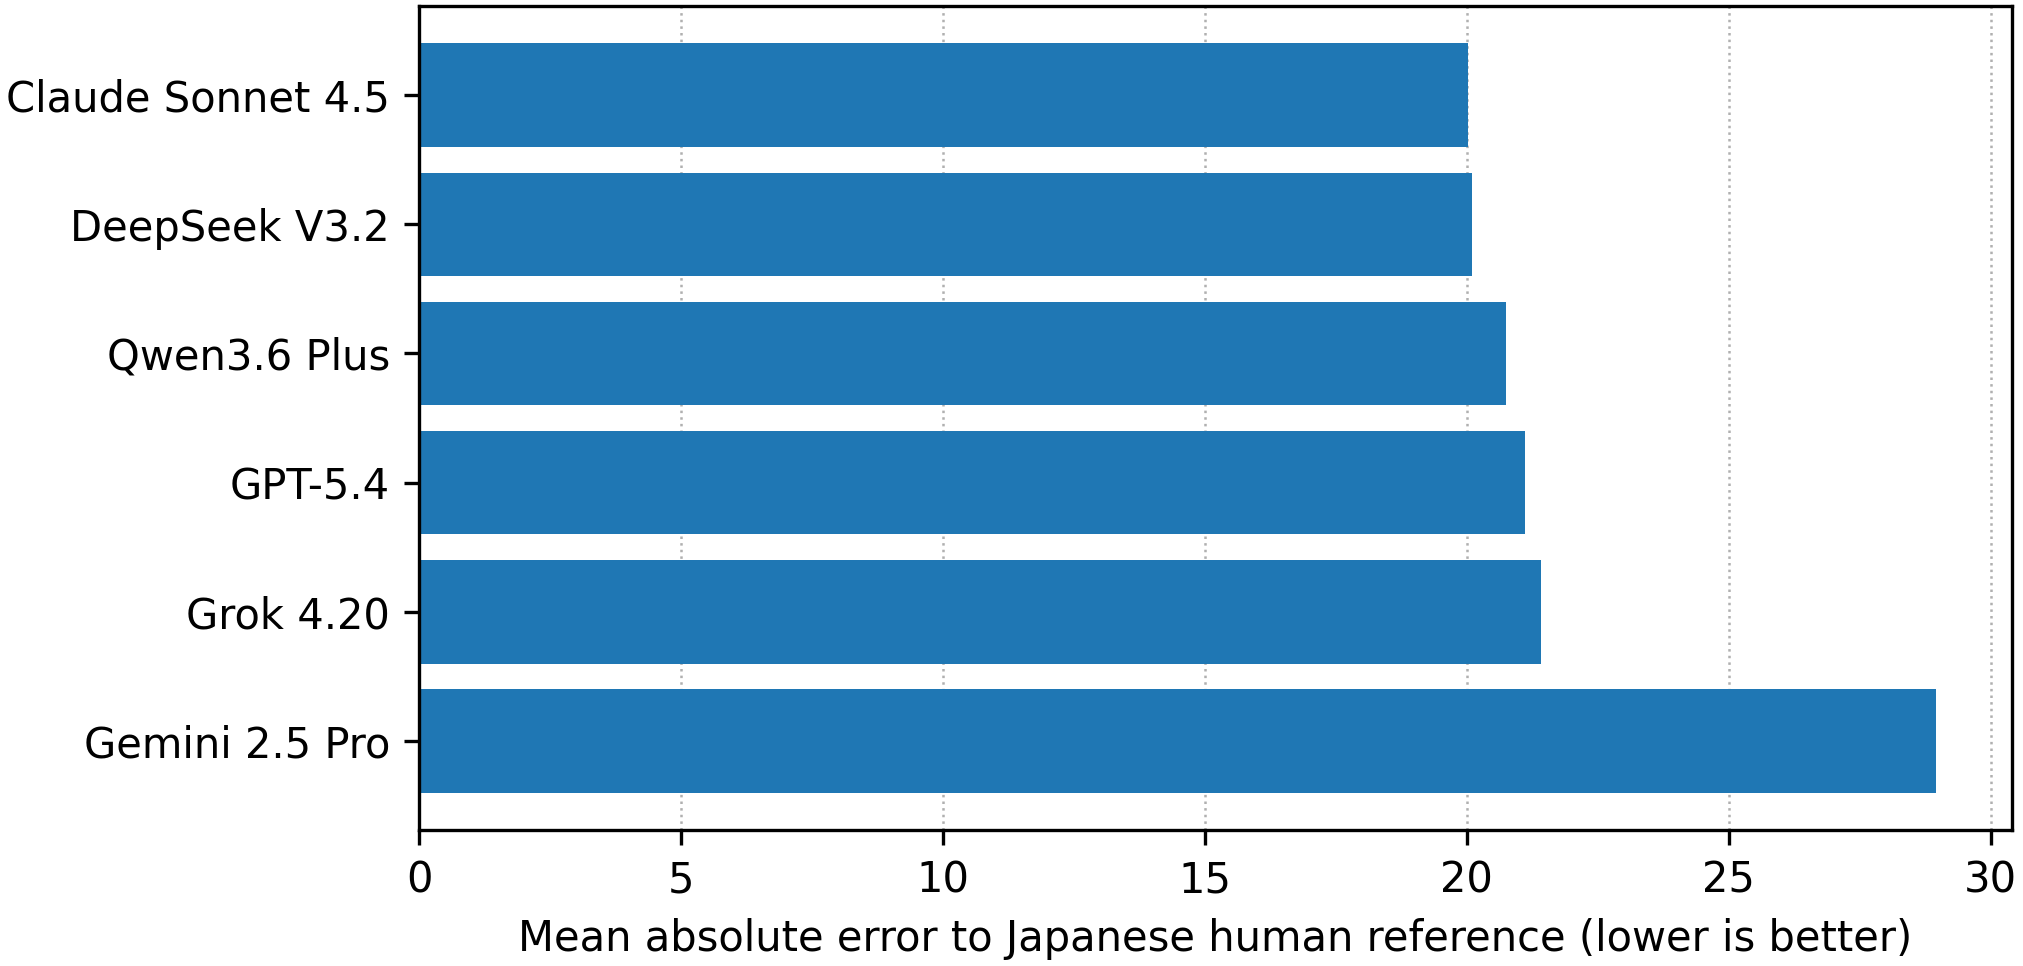
\includegraphics[width=0.95\textwidth]{fig/figure2_ja_ranking.pdf}
\caption{中立的読者条件における、選定6モデルの日本語人間整合性ランキング。モデルは日本語人間参照に対する平均絶対誤差（MAE）の小さい順に並べている。値が小さいほど、人間のVAS判断に近いことを示す。相関係数は表~\ref{tab:primary}に別途示す。}
\label{fig:ja-ranking}
\end{figure}

GPT-5.4は、日本語人間プロファイルとのPearson相関が最も高く（$r = 0.475$）、Spearman順位相関も最も高かった（$\rho = 0.441$）。この分離は重要である。絶対的な較正と順位の一致は、単一のスコアにまとめるのではなく区別して扱うべきだからである。Claude Sonnet 4.5は絶対的な感情強度水準において最も近く、GPT-5.4は12個の人間参照セルにわたる相対的な順序を最もよく保持していた。

\textbf{言語横断ロバスト性.}
言語横断ロバスト性については、Qwen3.6 Plusが日本語に対する平均ドリフトで最小（$\bar{D}=3.346$）を示し、GPT-5.4（$\bar{D}=3.354$）とGemini 2.5 Pro（$\bar{D}=4.729$）がこれに続いた。一方、DeepSeek V3.2は最大の平均ドリフト（$\bar{D}=6.396$）を示し、単一言語条件で最大のドリフトは同モデルの英語条件（7.875）で観測された。すべてのモデルおよび副次言語にわたり、ドリフトは2.983から7.875点の範囲にあった。

\begin{figure}[t]
\centering
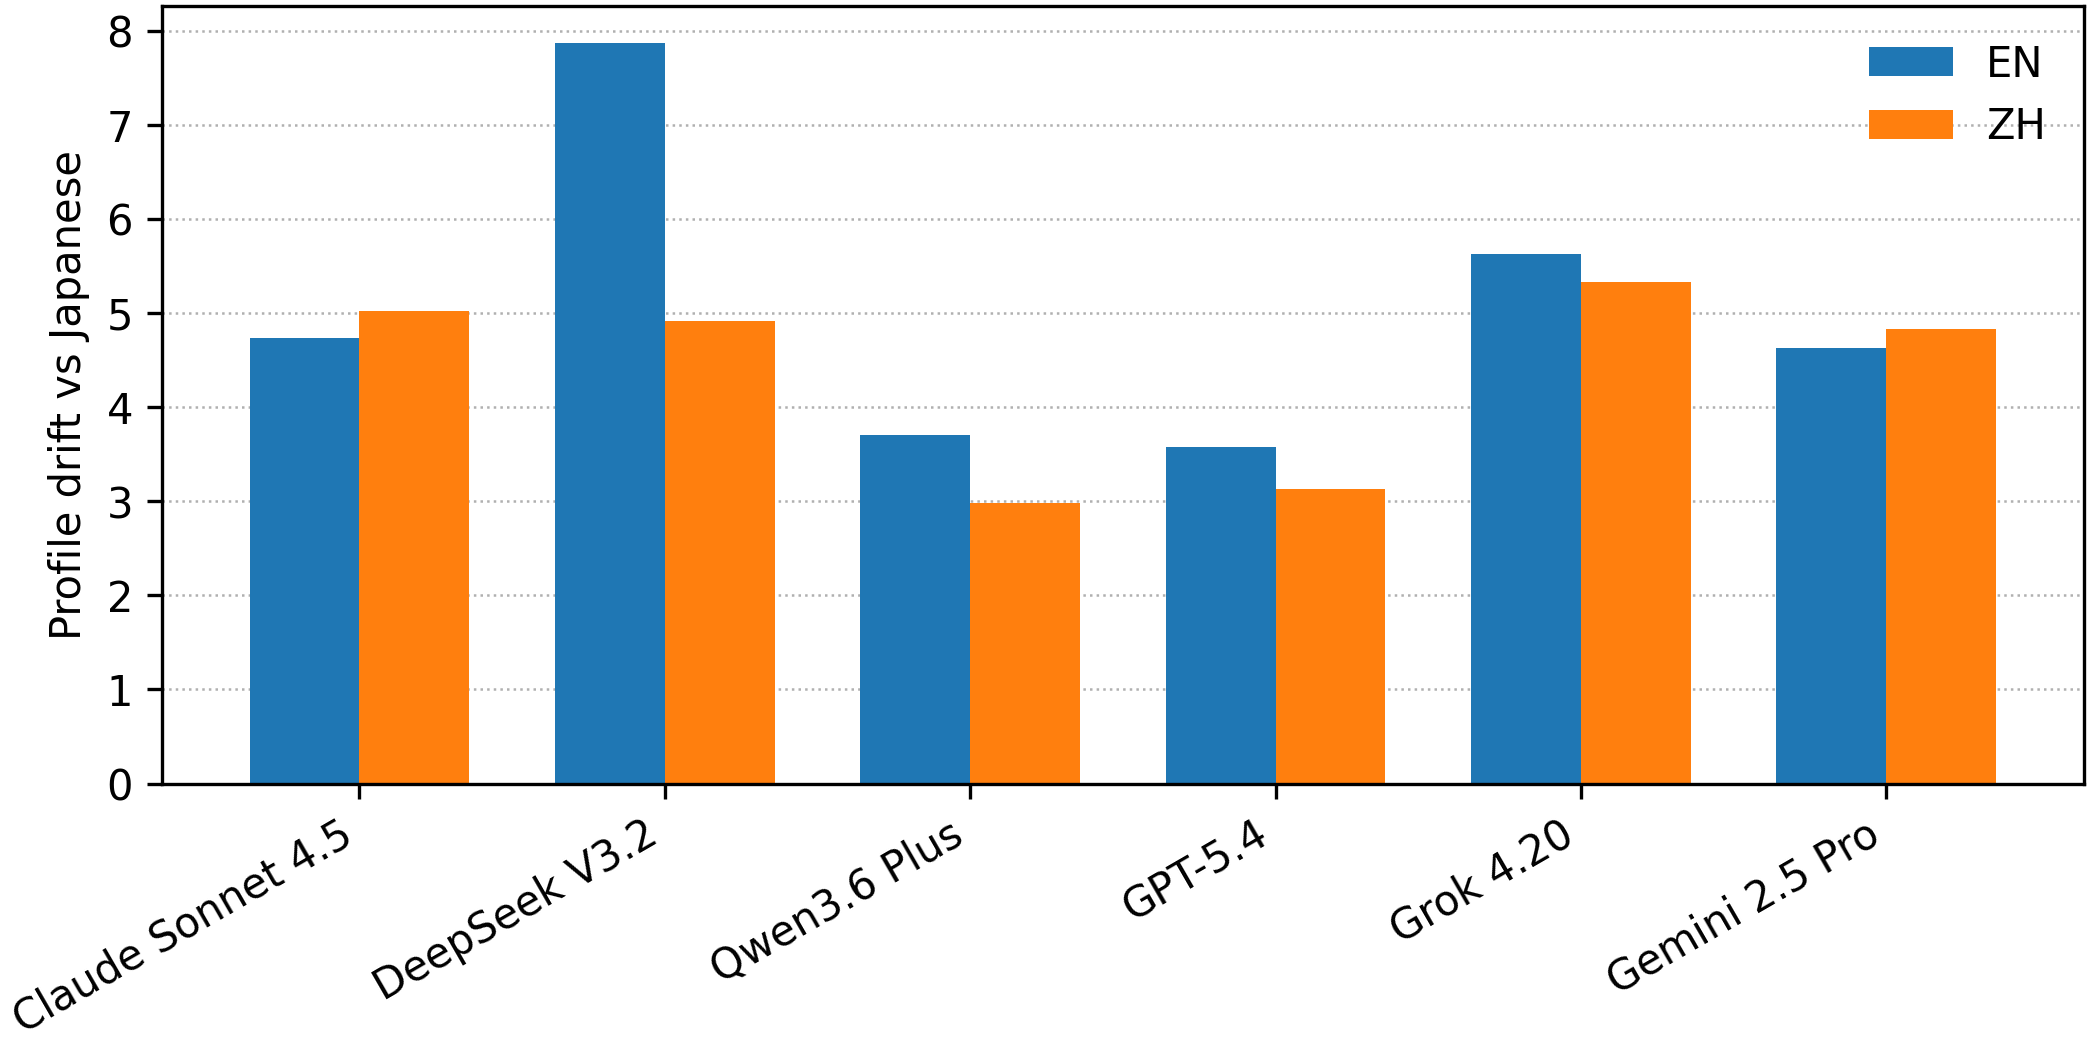
\includegraphics[width=0.95\textwidth]{fig/figure3_cross_language_drift.pdf}
\caption{中立的読者条件における、選定6モデルの日本語に対する言語横断ドリフト。ドリフトは、各モデルの英語または中国語の物語別・感情別スコアプロファイルと、同じモデルの日本語プロファイルとの平均絶対差として定義される。値が小さいほど、言語横断ロバスト性が高いことを示す。}
\label{fig:drift}
\end{figure}

この6モデルのパネルでは、英語条件は中国語条件よりも平均的にやや不安定であった。平均英語ドリフトは5.024であり、平均中国語ドリフトは4.371であった。この差は推論統計上の主張ではなく記述的な結果であるが、それでも翻訳条件におけるロバスト性が言語間で対称であるとは仮定できないことを示している。

\begin{table}[t]
\caption{選定6モデルにおける日本語人間整合性と言語横断ドリフトの主要定量要約}
\label{tab:primary}
\centering
\small
\begin{tabular}{lrrrrrr}
\toprule
モデル & JA MAE & JA Pearson $r$ & JA Spearman $\rho$ & EN drift & ZH drift & 平均drift \\
\midrule
Claude Sonnet 4.5 & 20.026 & 0.442 & 0.252 & 4.733 & 5.025 & 4.879 \\
DeepSeek V3.2 & 20.100 & 0.459 & 0.301 & 7.875 & 4.917 & 6.396 \\
Qwen3.6 Plus & 20.744 & 0.374 & 0.214 & 3.708 & 2.983 & 3.346 \\
GPT-5.4 & 21.113 & 0.475 & 0.441 & 3.575 & 3.133 & 3.354 \\
Grok 4.20 & 21.410 & 0.305 & 0.112 & 5.625 & 5.333 & 5.479 \\
Gemini 2.5 Pro & 28.952 & 0.261 & 0.112 & 4.625 & 4.833 & 4.729 \\
\bottomrule
\end{tabular}
\end{table}

\textbf{二軸スクリーニング視点.}
日本語ランキングとドリフトランキングは関連しているが、同一ではない。Claude Sonnet 4.5は日本語で最もよく較正されたモデルである一方、Qwen3.6 Plusは最小の平均言語横断ドリフトを示した。Gemini 2.5 Proは日本語MAEが最大であり、DeepSeek V3.2は平均ドリフトが最大であった。図~\ref{fig:tradeoff}は、日本語人間整合性MAEと平均EN/ZHドリフトをプロットすることで、この分離を明示している。

\begin{figure}[t]
\centering
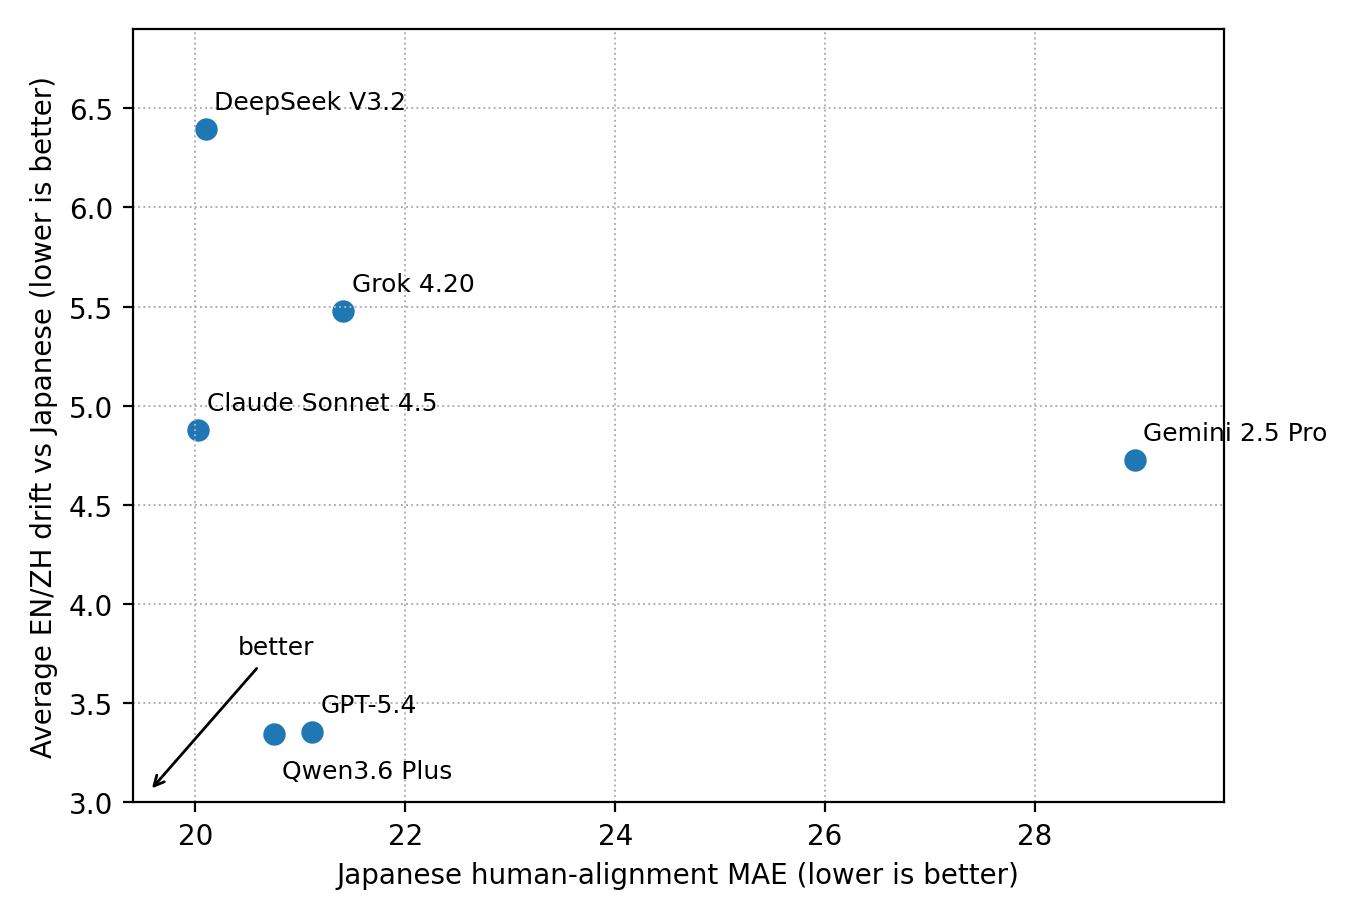
\includegraphics[width=0.82\textwidth]{fig/figure4_alignment_vs_avg_drift.pdf}
\caption{本ベンチマークの二軸スクリーニング視点。横軸は日本語人間整合性MAE、縦軸は日本語に対する平均EN/ZHドリフトを示す。主要言語での較正と多言語ロバスト性の双方が重要な場合、左下の領域が望ましい。}
\label{fig:tradeoff}
\end{figure}

両軸で単独に優位なモデルは存在しなかった。Claude Sonnet 4.5は主要な人間評価基盤エンドポイントで最も強く、Qwen3.6 PlusとGPT-5.4は多言語安定性で最も強く、Gemini 2.5 Proは中程度のロバスト性が弱い主要言語整合性を補償しないことを示している。この分離は、展開を意識した評価にとって重要である。モデルは主要言語における人間の感情強度水準に比較的よく整合していても、翻訳条件下では異なる安定性を示すことがあり、その逆もあり得る。

\section{考察}

これらの結果から3点が導かれる。第一に、多言語変動は人間妥当性と同じではない。モデルは多言語プロンプティングのもとで一見もっともらしく見えても、日本語人間参照と直接比較して較正を評価すると、大きく乖離する可能性がある。これが、日本語人間整合性を主要評価項目とし、EN/ZHの挙動を同等の人間評価基盤評価ではなくロバスト性分析として扱う主な理由である。

第二に、コンパクトなベンチマークでも、運用上有用なスクリーニング情報を得ることができる。主要な日本語条件では、Claude Sonnet 4.5が人間参照に対する最小MAE（20.026）を達成し、上位4モデルはわずか1.087 MAE点の範囲内にあった。一方、GPT-5.4は日本語Pearson相関およびSpearman相関が最も高く（0.475および0.441）、絶対的な較正と順位一致を単一スコアにまとめず区別すべきであることを示している。多言語ロバスト性では、Qwen3.6 PlusとGPT-5.4が最小の平均EN/ZHドリフト（3.346および3.354）を示し、DeepSeek V3.2は最大の平均ドリフト（6.396）を示した。したがって、人間整合性と多言語ロバスト性の両方を支配する単一モデルは存在しなかった。

\begin{table}[t]
\caption{6モデルパネルの実用的スクリーニング解釈}
\label{tab:screening}
\centering
\small
\begin{tabular}{@{}p{0.25\textwidth}p{0.33\textwidth}p{0.32\textwidth}@{}}
\toprule
モデル & 強み & 注意点 \\
\midrule
Claude Sonnet 4.5 & 日本語MAEが最良 & 平均多言語ドリフトは中位程度 \\
DeepSeek V3.2 & 日本語MAEが2番目に良好 & 平均ドリフトが最大で、英語が特に不安定 \\
Qwen3.6 Plus & EN/ZH平均ドリフトが最小 & 日本語整合性は上位2モデルに及ばない \\
GPT-5.4 & 日本語PearsonおよびSpearmanが最高で、平均ドリフトもほぼ最良 & 日本語MAEは最小ではない \\
Grok 4.20 & 両軸で中位 & 6モデルパネル内で首位の指標がない \\
Gemini 2.5 Pro & 平均ドリフトは中程度 & パネル内で日本語MAEが最大 \\
\bottomrule
\end{tabular}
\end{table}

表~\ref{tab:screening}は、同じ点を運用上の観点から要約している。本ベンチマークは単一の支配的モデルを特定するものではなく、各モデルがどのようなトレードオフを示しているかを、コンパクトで検討可能な形式で明らかにする。このため、本プロトコルは、より大規模な検証キャンペーンを開始する前の初期段階のモデル絞り込みに有用である。

第三に、本論文は、今回のICECCME向け貢献が我々の先行するLLMのみのフレームワーク論文とどのように異なるかを明確にする。先行研究は、36モデルの広範なモデル群において、ペルソナに割り当てた温度条件下で感情的個性を特徴づけることを目的としていた\cite{shirahama2026mdpi}。これに対して本論文は、中立的読者の主要条件を固定し、人間整合性を主要評価項目として用いる。この転換により、本論文は多次元的な個性分析ではなく、ベンチマーク設計と言語横断ロバスト性に焦点を当てた、コンパクトな工学系会議論文としてより適したものとなっている。

この中立的読者制約は、単なる文体上の制約ではなく方法論的制約である。ロールプレイや創造性プロンプトを導入すると、スコア変化がより良い人間整合性を反映しているのか、異なる解釈姿勢を反映しているのか、あるいはプロンプト誘発の分散を反映しているのかを判断しにくくなる。人間評価基盤のパイロットベンチマークでは、主要評価項目を一つの中立条件に固定することで、プロバイダ横断の比較を解釈しやすく、再現しやすくできる。より豊かなペルソナ条件付き評価は依然として有用であるが、それは安定した人間参照ベースラインを置き換えるのではなく、その上に段階的に重ねるべきである。

本ベンチマークは、展開認証ではなく第1段階のフィルタとして理解すべきである。主な限界は、3テキスト、1つの日本語学生読者参照条件、1つの中立的読者主要実行のみを用いている点である。英語と中国語は人間評価基盤のエンドポイントではなくロバスト性条件であり、測定されたドリフトは指示言語のみではなく、翻訳された文学テキストと言語を一致させた課題指示の双方を反映する。分析は、形式的な有意性検定ではなく、スクリーニング有用性のための記述的比較である。データ収集時には、トランスポートおよびスキーマ層でプロバイダ互換性の調整も必要であったが、課題定義、原文テキスト、スコアリング次元は固定した。次の段階では、テキスト数の増加、より大きな人間参照サンプル、英語および中国語に対応した人間参照という順序で、新たな証拠を制御しながら積み重ねる必要がある。

\section{結論}

本論文では、現代的な大規模言語モデルにおける文学的感情評価のために、コンパクトな人間評価基盤の多言語ベンチマークを提示した。学生読者による日本語VAS参照を用い、中立的読者プロンプトのもとで6つの現行モデルを比較した結果、Claude Sonnet 4.5が日本語人間プロファイルとの絶対的な一致において最も近く、GPT-5.4が最も強い順位一致を示し、Qwen3.6 Plusが最小の平均言語横断ドリフトを示した。より広く見れば、これらの結果は、主要な人間整合性と多言語ロバスト性が関連しつつも分離可能な性質であることを示している。したがって、今後のLLM感情評価研究では、これらを独立に報告し、より大規模な多言語評価またはマルチペルソナ評価の前段階として、コンパクトな人間評価基盤ベンチマークを初期スクリーニングに用いることを推奨する。

\section*{謝辞}

本論文は、より広範なEQ-Fuzzy研究プログラムの中で開発された、コンパクトな人間評価基盤ベンチマーク設計を用いている。著者らは、日本語VAS研究に参加した学生読者に感謝するとともに、実験刺激として青空文庫テキストを使用したことをここに記す。

本研究の一部は、日本学術振興会科学研究費助成事業（JSPS KAKENHI）課題番号26K14983および24K13350の支援を受けた。

\begin{thebibliography}{00}

\bibitem{shirahama2025vas}
N. Shirahama, N. Nakaya, S. Watanabe, et al., ``Assessing Emotional Intelligence in AI: Visual Analogue Scale vs. Likert Scale in Short Story Comprehension,'' \emph{Journal of the Institute of Industrial Applications Engineers}, vol. 13, no. 1, pp. 21--31, 2025.

\bibitem{shirahama2026mdpi}
N. Shirahama, Y. Yoshimoto, N. Nakaya, and S. Watanabe, ``Mathematical Framework for Characterizing Emotional Individuality in Large Language Models: Temperature Control, Fuzzy Entropy, and Persona-Based Diversity Analysis,'' \emph{Mathematics}, vol. 14, no. 7, Art. no. 1224, 2026.

\bibitem{paech2024eqbench}
S. J. Paech, ``EQ-Bench: An Emotional Intelligence Benchmark for Large Language Models,'' arXiv:2312.06281, 2024.

\bibitem{huang2024emotionbench}
J. Huang, M. H. Lam, E. J. Li, S. Ren, W. Wang, W. Jiao, Z. Tu, and M. R. Lyu, ``Emotionally Numb or Empathetic? Evaluating How LLMs Feel Using EmotionBench,'' arXiv:2308.03656, 2024.

\bibitem{sabour2024emobench}
S. Sabour, S. Liu, Z. Zhang, J. Liu, J. Zhou, A. Sunaryo, T. M. C. Lee, R. Mihalcea, and M. Huang, ``EmoBench: Evaluating the Emotional Intelligence of Large Language Models,'' in \emph{Proc. 62nd Annual Meeting of the Association for Computational Linguistics (ACL)}, 2024, pp. 5986--6004.

\bibitem{chen2024emotionqueen}
Y. Chen, S. Yan, S. Liu, Y. Li, and Y. Xiao, ``EmotionQueen: A Benchmark for Evaluating Empathy of Large Language Models,'' in \emph{Findings of the Association for Computational Linguistics: ACL 2024}, 2024, pp. 2149--2176.

\bibitem{openrouterplatform}
N. Shirahama, N. Nakaya, and S. Watanabe, ``Development of an Experimental Platform for Evaluating LLM Emotion Understanding,'' \emph{ICIC Express Letters}, vol. 20, pp. 191--198, 2026.

\end{thebibliography}

\end{document}
